%! Author = Vojta
%! Date = 25.11.2021

\chapter{Testování}

Pod pojmem testování si člověk může představit široké spektrum možností. Může to být automatizované testování při nahrání kódu
do verzovacího systému a následném sestavení nebo například penetrační testování. Já jsem zvolil pouze uživatelské testování,
které mi pomůže porozumět, jak nový uživatel aplikaci vnímá a zda jsou v ní nějaká problematická místa, které je potřeba ještě
poupravit.

\section{Uživatelské testování}
Tento typ testování se především provádí při prvním vydání dané aplikace. Pro lepší popis se dá použít výraz testování použitelnosti,
tedy zkouška, zda aplikace neobsahuje nějaké větší problémy, které by uživatelům bránily v jejím použití~\cite{UserTesting}. Je díky tomu možné
zjistit, jak se chová běžný uživatel, který aplikaci nikdy předtím neviděl. Tím pádem tento typ testu nemůže provádět vývojář,
který aplikaci již velmi dobře zná.

\subsection{Nejčastější problémy které se při testování objeví}

Podle článku \textbf{Jak dělat uživatelské testování}~\cite{UserTesting} se nejčastěji narazí na:

\begin{itemize}
    \item Špatně nazvané prvky -- pro uživatele není jasné, co si pod daným prvkem představit
    \item Špatně dohledatelné informace -- uživatel nenajde chtěnou informaci na místě, kde by měla být
    \item Hůře dostupné prvky -- uživatel má potíže se k danému prvku dostat
    \item Neodpovídající obsah -- uživatel očekává jiné informace, než ty které se na stránce skutečně nacházejí
    \item Nestandardní chování prvků -- např. tlačítko zobrazující šipku zpět má jinou funkci než vrácení na poslední stránku
\end{itemize}

\subsection{Otestování grafického návrhu}

Tento test lze provést nad návrhem, který jsem vytvářel v aplikaci Adobe XD. Jelikož tato aplikace umožňuje prototyp tvořit interaktivně,
je poté možné nasimulovat webovou aplikaci, kterou si uživatel může proklikat. Nakonec jsem pouze prodiskutoval problematická místa s vedoucím a rozhodl jsem
se, že plně otestuji implementovanou aplikaci, která přinese více prvků, se kterými jsem v návrhu nepočítal nebo musely být změněny.

\subsection{Příprava před testem}

Nejdříve bylo potřeba vybrat vhodné uživatele na testování (dále respondenti). To nebyl velký problém, jelikož jsem se domluvil s většinou potencionálních
uživatelů, se kterými jsem prováděl kvalitativní průzkum, zda by měli zájem o finální testování, popřípadě používání aplikace.
Vzhledem k tomu, že v době kdy jsem udělal průzkum bylo typické dělat schůzky online, ponechal jsem to tak i v tomto případě.
Jako hlavní výhodu jsem vnímal, že nebudu muset koukat respondentům přes rameno a budu si moct průběh testu nahrát a případně se
k záznamu vrátit.

Připravil jsem si tedy scénář, který je provedl celou aplikací, tak jako by to uživatel, který chce aplikaci začít používat udělal.
Snažil jsem se dávat otázky či úkoly, které nebyly tolik navádějící, ačkoliv v některých případech to nebylo možné.

\subsubsection{Scénář použitý při testování}
\begin{itemize}
    \item Otevřete si stránku recipeo.cz
    \item Popište, kde se právě nacházíte
    \item Zobrazte stránku s recepty
    \item Zvolte recept, který se vám líbí a otevřete jej
    \item Co byste udělal, kdybyste chtěl vařit pro dva lidi?
    \item Zobrazte stránku s ingrediencemi
    \item Zvolte jednu ingredienci a otevřete ji
    \item Popište, kde se nacházíte a jaké informace o ingredienci vidíte
    \item Přihlašte se do aplikace
    \item Přidejte novou ingredienci
    \item Přidejte nový recept a použijte v něm dříve vytvořenou ingredienci
    \item Představte si, že jste v receptu či ingredienci udělal chybu a musíte jej upravit, jak toho dosáhnete?
    \item Chcete si připravit seznam receptů, které budete vařit příští týden, co uděláte?
    \item Naopak nechcete nic plánovat, ale nevíte co si rychle uvařit, zkuste najít, co by vám v aplikaci pomohlo
    \item Přidejte novou skupinu a pozvěte mě do ní
    \item Připojte se do následující skupiny
    \item Co vás na stránkach zaujalo a co se vám naopak nelíbilo?
\end{itemize}

Po dokončení scénáře jsem ještě respondenty poprosil, aby se v prohlížeči přepnuli do mobilního zobrazení a aplikaci si zkusili proklikat.

\section{Průběh testu}

Všechny testy proběhly v rámci jednoho týdne. Mezi testy jsem se snažil předělat problémová místa tak, abych od dalšího respondenta dostal
nové informace a odpovědi se neopakovaly. Na nejvíce problému respondenti narazili v horní liště aplikace. Prvky totiž obsahovaly \emph{hover}
efekt, tedy otevřely skryté menu po najetí myši. Tím se pro uživatele zhoršila orientace po aplikaci a některé stránky tak zůstaly úplně skryty.
Problém jsem vyřešil tím, že jsem přidal tlačítka se stejnou funkcí na další místa v aplikaci. Například odkaz na přidání receptu jsem přidal
na stránku s recepty nebo odkaz na skupiny na stránku účtu.

\begin{figure}[H]
    \centering
    \subfloat[Schovaný odkaz na přidání receptu]{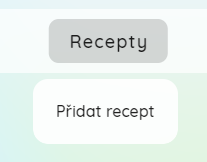
\includegraphics[width=0.4\textwidth]{images/recipeo-hover}\label{picture:recipeo:hover}}
    \hfill
    \subfloat[Přidaný viditelný odkaz u seznamu receptů]{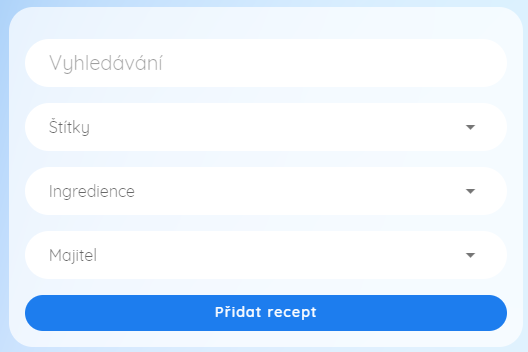
\includegraphics[width=0.5\textwidth]{images/recipeo-add-button}\label{picture:recipeo:add-button}}
    \caption{Nalezené problémové místo a následná úprava}
\end{figure}

Další problém jsem našel hned s prvním respondentem. Bylo jím špatně navržené přepínání účtů. V horní liště byla zobrazena ikona s iniciály uživatele
popřípadě aktivní skupiny. Po najetí na ikonu se zobrazilo menu, kde si uživatel mohl vybrat mezi svým účtem a skupinami, ve kterých je členem. To
ovlivnilo i další místa v aplikaci jako zobrazení receptů nebo přidání receptu. To mohlo být pro uživatele, který o tomto nevěděl velmi matoucí, a
tak jsem se rozhodl prvky rozdělit a přidat do míst která ovládaly. Z lišty jsem tedy přesunul volbu uživatele k přidání receptu jako \emph{autocomplete}
a taktéž jsem učinil u filtrování receptů.

Dále jsme zjistili, že v některých situacích se nesprávně načítají data. Například při prvním spuštění aplikace a následovném přidání ingredience
se nenačetla její stránka. Nebo při přijmutí pozvánky do skupiny se nenačetly recepty, které skupina obsahuje.

Při přihlášení byl uživatel pouze přesměrován na úvodní stránku. To se všem respondentům zdálo jako nedostatečné upozornění na danou událost.
Přidal jsem tedy \emph{alert} z knihovny Vuetify, který by měl uživateli dát dostatečně najevo co se děje.

Jak jsem psal výše, na konci scénáře jsem s respondenty prošel aplikaci v mobilním zařízení. Dva z nich měli problém s akcí vrácení se na předchozí stránku,
tedy tlačítko zpět. Ovšem myslím si, že toto byl falešný poplach, způsobený tím, že test byl prováděn na počítači a mobilní zobrazení bylo pouze simulované.
Vzhledem k tomu, že se aplikace tváří jako nativní, uživatel by měl pro navigaci po aplikaci využívat prvky operačního systému, tedy šipku zpět v liště nebo
v novějších zařízeních gesto ze strany displeje.

\section{Vyhodnocení výsledků}

Vzhledem k nízkému počtu chyb v uživatelském rozhraní si dovolím říct, že \emph{frontend} aplikace testem použitelnosti prošel. Až na některé
skryté prvky, které jsem jednoduše naduplikoval na viditelnější místa, neměli testeři žádné problémy s navigací po aplikaci či využití
všech jejích funkcí. Design aplikace také všichni hodnotili pozitivně, což splňuje cíl, který jsem si stanovil při jeho návrhu. Tedy aby
se aplikace uživatelům líbila, působila moderně a byla srozumitelná.

Co se týče funkčnosti, zde to bylo horší a nejvíce problému se objevilo při stahování dat z databáze. Někdy nastaly situace, kde se správně
neaktualizovala data, a tak uživatel neměl přístup k veškerému obsahu. To ale nebyl problém spravit po nálezu míst, ve kterých se tyto nesrovnalosti
děly.
